\documentclass[../main.tex]{subfiles}
\begin{document}
\chapter{Higher Order Linear ODEs}
We will focus on 2nd order here, but many methods are also applicable to higher orders.
\section{Constant Coefficients}
The general form of a 2nd order linear ODE with constant coefficients is:
\begin{equation}
  \label{general2ndConst}
  \underbrace{a \deriv[2]{y}{x} + b \deriv{y}{x} + cy}_{\mathcal{D}y} = f(x)
\end{equation}
with $a, b, c$ constants.
Where $\mathcal{D}y$ is a linear differential operator, defined as:
\[
  \mathcal{D} \equiv a \deriv[2]{}{x} + b \deriv{}{x} + c
\]
\begin{definition}[Linear Operator]
  A differential operator, $\mathcal{D}$ is \textit{linear} if for any $y_1(x)$ and $y_2(x)$ and constants $\alpha$ and $\beta$:
  \[
    \mathcal{D}(\alpha y_1 + \beta y_2) = \alpha \mathcal{D}y_1 + \beta \mathcal{D}y_2
  \]
  This is also known as the \textit{principle of superposition}.
\end{definition}
We can exploit this property to solve \cref{general2ndConst}:
\begin{enumerate}
  \item Find complimentary functions (C.F.), $y_c$, that satisfy the corresponding homogeneous equation:
    \[
      a \deriv[2]{y_c}{x} + b \deriv{y_c}{x} + c y_c = 0
    \]
  \item Find \textbf{any} particular integral (P.I.), $y_p$ that satisfies the full equation.
  \item Then a solution of the full equation is then $y_c + y_p$ as:
    \[
      \mathcal{D}(y_c + y_p) = \underbrace{\mathcal{D}y_c}_{=0} + \mathcal{D}y_p = f(x)
    \]
    So it satisfies the full equation.
\end{enumerate}
A 2nd order ODE has \textbf{two} linearly independent complimentary functions, so the general solution to is:
\[
  y(x) = C_1 y_{c_1}(x) + C_2 y_{c_2}(x) + y_p(x)
\]
with $C_1, C_2$ constants.
\begin{definition}[Linear Dependance]
  A set of $n$ functions $\{f_i(x)\}$ is \textit{linearly dependant} if:
  \[
    \sum_{i=1}^{n} C_i f_i(x) = 0\ \forall x
  \]
  for $n$ constants, $C_i$, \textbf{not} all of which are $0$.
  Otherwise they are \textit{linearly independent}.
\end{definition}
\begin{remark}
  This is the same idea as linear dependence for vectors.
\end{remark}
Equivalently, if one or more of the functions $f_i(x)$  can be written as a linear combination of the others, they are linearly \textbf{dependant}.
\subsection{Complimentary Functions}
Recall that:
\[
  \deriv{}{x} e^{\lambda x} = \lambda e^{\lambda x} \text{ (Eigenfunction)}
\]
$e^{\lambda x}$ is also an eigenfunction of $\mathcal{D}$ because:
\begin{align*}
  \mathcal{D}(e^{\lambda x}) &= a \deriv[2]{}{x} e^{\lambda x} + b \deriv{}{x} e^{\lambda x} + c \\
                             &= \underbrace{(a\lambda^2 + b\lambda + c)}_{\text{eigenvalue}} e^{\lambda x}
\end{align*}
The complimentary functions of \cref{general2ndConst} satisfy $\mathcal{D}y_c = 0$, that is, they are eigenfunctions with eigenvalue $0$.
Thus:
\[
  y_c = A e^{\lambda x} \text{ with } \underbrace{a \lambda^2 + b\lambda + c = 0}_{\text{characteristic equation}}
\]
Since the characteristic equation of $\mathcal{D}$ is a 2nd degree polynomial it must have two roots $\lambda_1$ and $\lambda_2$.
\begin{proofcases}
  \begin{case}{$\lambda_1 \neq \lambda_2$}
    We then have two linearly independent complimentary functions:
    \[
      y_{c_1} \propto e^{\lambda_1 x}, y_{c_2} \propto e^{\lambda_2 x}
    \]
    So the most general complimentary function is a linear combination:
    \[
      y_c = C_1 y_{c_1}(x) + C_2 y_{c_2}(x)
    \]
    So $y_{c_1}$ and $y_{c_2}$ for a \textit{basis} for the space of solutions for the homogeneous equation.
    Note that if the roots are complex, we get oscillatory behaviour.
  \end{case}
  \begin{case}{$\lambda = \lambda_2$ -- Degenerate Case}
    So now we have only one linearly independent complimentary function of the form $e^{\lambda_1 x}$.
    See \cref{detuningExample} for how to deal with this case.
  \end{case}
\end{proofcases}
\begin{example}[Real, non-degenerate roots]
  \[
    \deriv[2]{y}{x} - 5\deriv{y}{x} + 6y = 0
  \]
  The characteristic equation is then:
  \[
    \lambda^2 - 5\lambda + 6 = 0 \implies \lambda_1 = 3, \lambda_2 = 2
  \]
  So the general complimentary function is:
  \[
    y_c(x) = A e^{3x} + B e^{2x}
  \]
  with $A, B$ constants.
\end{example}
\begin{example}[Complex, non-degenerate roots]
  \label{complexNonDegenerate}
  \[
    \deriv[2]{y}{x} + 4y = 0
  \]
  The characteristic equation is then:
  \[
    \lambda^2 + 4 = 0 \implies \lambda_1 = 2i, \lambda_2 = -2i
  \]
  So the general complimentary function is:
  \[
    y_c(x) = Ae^{2ix} + Be^{-2ix}
  \]
  Note that $e^{\pm2ix} = \cos(2x) \pm i \sin(2x)$ so:
  \begin{align*}
    y_c(x) &= (A + B)\cos(2x) + (A - B)i\sin(2x) \\
           &= \alpha \cos(2x) + \beta \sin(2x)
  \end{align*}
  Whether $\alpha, \beta$ are complex depends on the boundary conditions of the problem.
\end{example}
\begin{example}[Degenerate roots and ``detuning'']
  \label{detuningExample}
  \[
    \deriv[2]{y}{x} - 4\deriv{y}{x} + 4y = 0
  \]
  So the characteristic equation is:
  \[
    \lambda^2 - 4y + 4 = 0 \implies \lambda = 2
  \]
  Therefore we have degenerate roots and only one linearly independent complimentary function $e^{2x}$.

  \textbf{Detuning - }Remove the degeneracy by considering a slightly modified (\textit{detuned}) equation.
  \[
    \deriv[2]{y}{x} - 4 \deriv{y}{x} + (4 - \varepsilon^2)y = 0 \quad (\varepsilon \ll 1)
  \]
  So the characteristic equation is now:
  \[
    \lambda^2 - 4\lambda + (4 - \varepsilon^2) = 0 \implies \lambda = 2 \pm \varepsilon
  \]
  Which gives the complimentary function:
  \begin{align*}
    y_c(x) &= Ae^{(2 + \varepsilon)x} + Be^{(2 - \varepsilon)x} \\
           &=e^{2x}(Ae^{\varepsilon x} + Be^{-\varepsilon x}) \\
           &=e^{2x}[(A+B) + \varepsilon(A - B)x + O(A\varepsilon^2x^2) + O(B\varepsilon^2x^2)] \text{ (as $\varepsilon \to 0$)} \\
  \end{align*}
  Apply the initial conditions $y(0) = C$ and $y'(0) = D$ to both the original and detuned equations.
  This yields the equations:
  \begin{align*}
    &A + B = C \text{ and } 2C + \varepsilon(A - B) = D \\
    \implies& A = \frac{1}{2}\left(C + \frac{D - 2C}{\varepsilon}\right),\ B = \frac{1}{2}\left(C - \frac{D - 2C}{\varepsilon}\right)
  \end{align*}
  So $O(A) \text{ and } O(B) = O(\frac{1}{\varepsilon})$ as $\varepsilon \to 0$.
  Therefore $O(A\varepsilon^2x^2) \text{ and } O(B\varepsilon^2x^2) = O(\varepsilon x^2) \to 0$ as $\varepsilon \to0$.

  Now let:
  \[
    \alpha = A + B, \beta = \varepsilon(A - B)
  \]
  Both $\alpha$ and $\beta$ are $O(1)$ as they do not depend on $\varepsilon$ so are unchanged as $\varepsilon \to 0$.
  As we take $\varepsilon \to 0$, the detuned equation becomes the original equation, so the general solution of the original degenerate equation is:
  \[
    y = \alpha e^{2x} + \beta x e^{2x}
  \]
\end{example}
\begin{remark}[Note]
  In general, if $y_{c_1}$ is a degenerate complimentary function of a linear ODE with constant coefficients then $y_{c_2} = x y_{c_1}$ is a second linearly independent complimentary function.
\end{remark}
\section{Homogeneous Second Order ODEs with Non-constant Coefficients}
The general form of a homogeneous second order ODE with non-constant coefficients is:
\[
  y'' + p(x)y' + q(x)y = 0
\]
\subsection{Second Complimentary Function -- Reduction of order}
The following method allows us to find a second solution, $y_2(x)$, given one solution, $y_1(x)$.

We try a solution of the form $y_2(x) = v(x)y_1(x)$.
Therefore:
\[
  y_2' = v'y_1 + vy_1' \text{ and } y_2'' = v''y_1 + 2v'y_1' + vy_1''
\]
If $y_2$ satisfies the original ODE then we require that:
\begin{align*}
  v''y_1 + v'(2y_1' + py_1) + v(\underbrace{y_1'' + py_1' + qy_1}_{0}) &= 0 \\
  v''y_1 + v'(2y_1' + py_1) &= 0
\end{align*}
We can then let $u = y'$ to reduce the order of the DE:
\[
  u'y_1 + u(2y_1' + py_1) = 0
\]
This is now a separable first order ODE for $u$.
\begin{align*}
  \frac{u'}{u} &= -\frac{2y_1'}{y_1} - p \\
  \implies \ln u &= -2 \ln y_1  - \int_{0}^{x} p(t) \d{t} + \ln A \\
  \implies u(x) &= \frac{A}{y^{2}_{1}}\exp\left[-\int_{0}^{x} p(t) \d{t}\right]
\end{align*}
We can then, in theory, integrate this expression for $u(x)$ to obtain $v(x)$.
\begin{example}
  Consider again the DE from \cref{detuningExample}:
  \[
    y'' - 4y' + 4y = 0
  \]
  So $p(x) = -4, q(x) = 4$.
  We know that one solution is $y_1(x) = e^{2x}$.
  \[
    \frac{u'}{u} = -\frac{4e^{2x}}{e^{2x}} - (-4) = 0
  \]
  So $u$ and therefore $v'$ are constants so:
  \[
    v(x) = Ax+B
  \]
  Therefore we have a second solution $y_2$ given by:
  \[
    y_2(x) = (Ax + B)e^{2x}
  \]
  The $Be^{2x}$ replicates $y_1$ so $xe^{2x}$ is a second linearly independent solution.
\end{example}
\subsection{Phase Space}
The general form of an $n$-th order linear ODE is:
\[
  y^{(n)} + p(x)y^{(n-1)} + \cdots + q(x)y = f(x)
\]
This means that $y^{(n)}$ is determined by $y^{(0)}, \ldots, y^{(n-1)}$.
When we differentiate the equation, we see that higher order derivatives can also be determined by $y^{(0)}, \ldots, y^{(n-1)}$.
This means that we can construct a Taylor series about $x_0$ if we specify $y^{(0)}(x_0), \ldots, y^{(n-1)}(x_0)$.

In other words, the \textit{state of the system} is fully specified at any $x$ by an $n$-dimensional \textit{solution vector}:
\[
  \vec{Y}(x) = \begin{pmatrix}
  y(x) \\
  y^{(1)}(x) \\
  \vdots \\
  y^{(n-1)}(x) \\
  \end{pmatrix}
\]
That is, given such a $\vec{Y}(x_0)$ at any fixed $x_0$, we can determine the Taylor series for the solution and use this to determine $y$ and all of its derivatives at any $x$.
\begin{remark}
  \begin{itemize}
    \item At any $x$, $\vec{Y}(x)$ defines a point in $n$-dimensional \textit{phase space}.
    \item As $x$ varies, $\vec{Y}(x)$ traces a trajectory through \textit{phase space}.
  \end{itemize}
\end{remark}
\begin{example}
  Consider again the DE from \cref{complexNonDegenerate}:
  \[
    y'' + 4y = 0
  \]
  We know that $y_1(x) = \cos 2x$ and $y_2(x) = \sin 2x$ so the solution vectors are:
  \[
    \vec{Y}_1 = \begin{pmatrix}
    y_1 \\
    y_1' \\
    \end{pmatrix} =
    \begin{pmatrix}
    \cos 2x \\
    -2\sin 2x \\
    \end{pmatrix},\
    \vec{Y}_2 = \begin{pmatrix}
    y_2 \\
    y_2 \\
    \end{pmatrix} =
    \begin{pmatrix}
    \sin 2x \\
    2 \cos 2x \\
    \end{pmatrix}
  \]
  So in 2D phase space, $\vec{Y}_1$ and $\vec{Y}_2$ lie on the same ellipse:
  \begin{center}
  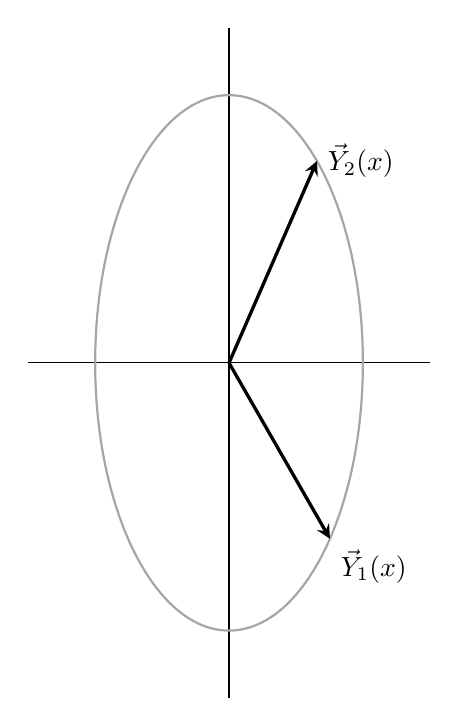
\begin{tikzpicture}[scale=1.7, >=stealth]
    \draw[-] (-1.5, 0) -- (1.5, 0);
    \draw[-] (0, -2.5) -- (0, 2.5);

    \draw[thick, gray!70] (0, 0) ellipse (1 and 2);

    \draw[->, very thick] (0, 0) -- (0.7539, -1.3139) node[below right] {$\vec{Y}_1(x)$};
    \draw[->, very thick] (0, 0) -- (0.6569, 1.5078) node[right] {$\vec{Y}_2(x)$};
  \end{tikzpicture}
  \end{center}
  $\vec{Y}_1$ and $\vec{Y}_2$ are linearly independent vectors.
  This means that they form a basis for the 2D phase space.
\end{example}
\section{Wronskian and Linear Dependence}
Recall that a set of functions $\{y_i(x)\}$ are linearly dependant if:
\[
  \sum_{i=1}^{n} c_i y_i(x) = 0\ \forall x,\ c_i \text{ not all 0}
\]
Since this holds for all $x$ we can differentiate it $1, 2, \ldots, n-1$  times.
Therefore:
\[
  \sum_{i=1}^{n} c_i y^{(k)}_i(x) = 0\ \forall x, k = 1, \ldots, n-1
\]
This sum the $k$-th entry in the sum of all the solution vectors, so we have:
\[
  \sum_{i=1}^{n} c_i \vec{Y}_i(x) = 0\ \forall x
\]
So if $\{y_i\}$ is linearly dependant, then $\{\vec{Y}_i(x)\}$ are linearly dependant for all $x$.

We can form a \textit{fundamental matrix}, $\Psi(x)$, whose columns are the solution vectors:
\[
  \Psi(x) = \begin{pmatrix}
  \uparrow & \uparrow &  & \uparrow \\
  \vec{Y}_1 & \vec{Y}_2 & \cdots & \vec{Y}_n \\
  \downarrow & \downarrow &  & \downarrow \\
  \end{pmatrix}
\]
\begin{definition}[Wronskian]
  The \textit{Wronskian} of $n$ functions $\{y_i\}$ is defined to be the following determinant:
  \[
    W(x) =
    \begin{vmatrix}
      y_1 & y_2 & \cdots & y_n \\
      y_1' & y_2' & \cdots & y_n' \\
      \vdots & \vdots & \ddots & \vdots \\
      y^{(n-1)}_1 & y^{(n-1)}_2 & \cdots & y^{(n-1)}_n \\
    \end{vmatrix}
  \]
\end{definition}
\begin{remark}[Note]
  In this case, the Wronskian is the determinant of the fundamental matrix, that is:
  \[
    W(x) =
    \det(\Psi(x)) =
    \begin{vmatrix}
      \uparrow & \uparrow &  & \uparrow \\
      \vec{Y}_1 & \vec{Y}_2 & \cdots  & \vec{Y}_n \\
      \downarrow & \downarrow &  & \downarrow \\
    \end{vmatrix}
  \]
\end{remark}
Recall that if a matrix has linearly dependant columns then its determinant is 0.
Therefore we have:
\[
  \{y_i(x)\} \text{ is linearly \textbf{dependant}} \implies \{\vec{Y}_i(x)\} \text{ is linearly \textbf{dependant}} \implies W(x) = 0\ \forall x
\]
Taking the contrapositive, it follows that if $W(x) \neq 0$ for some $x$ then $\{y_i(x)\}$ are linearly \textbf{independent}.
\begin{remark}[Warning]
  $W(x) = 0\ \forall x$  does \textbf{not} necessarily imply that $\{y_i(x)\}$ are linearly dependant.
\end{remark}
\begin{example}
  Consider again the DE from \cref{complexNonDegenerate}:
  \[
    y'' + 4y = 0
  \]
  We can calculate the Wronskian using the solution vectors we found earlier:
  \[
    W(x) = \begin{vmatrix}
    y_1 & y_2 \\
    y_1' & y_2' \\
    \end{vmatrix} = \begin{vmatrix}
    \cos 2x & \sin2x \\
    -2\sin 2x & 2\cos 2x \\
    \end{vmatrix}
    = 2(\cos^2 2x + \sin^2 2x) = 2
  \]
  Since $W(x) \neq 0\ \forall x$, $y_1$ and $y_2$ are linearly independent.
\end{example}
\section{Abel's Theorem}
\end{document}
